\documentclass[main.tex]{subfiles}

\begin{document}

\section{Photon Mapping} \label{section:pm}

Photon mapping is a ray tracing method that intends to approximate the rendering equation, first proposed as a global illumination technique in 1996 \cite{jensen1996global}, and works as a two-pass algorithm, working as an extension to ray tracing that allows the efficient computation of caustics\footnote{The light effects caused by light reaching a diffuse surface after being reflected or transmitted by a specular one} and indirect illumination of surfaces.

Unlike other algorithms such as Path Tracing or Metropolis Light Transport, this is a biased rendering method, meaning that a finite for a finite number of traced photons, the resulting estimation will always be different from the correct solution. However this can be worked around by increasing the size of the photon map structure used in the process, or by using variations of this technique, such as Stochastic Photon Mapping.

\subsection{Algorithm}

The original approach to photon mapping consists simply on a two step algorithm. One step to generate a structure with the illumination information for the scene, called the photon map, and a second step to trace rays from the camera to interact with the scene and the photon map, contributing to the final pixels of the generated image.

\image[width=\textwidth]{visio/diagram_pm}{High Level Flowchart of Photon Mapping}{fig:diagram_pm}

\subsubsection{First Step: Photon Map Construction}

In this step, a large number of photons must be traced, starting from the existing light sources in the scene (see \cref{fig:pm_step1}). The tracing of a photon is just like the tracing of a regular ray, interacting with the scene according to \acs{BRDF} function, in a process similar to path tracing. Every hit by a photon is stored in a structure called a photon map.
The original proposal \cite{jensen1996global} uses two different photon maps, the extra one being a higher density one used for the rendering of caustics. This is done by emitting paths towards specular objects in the scene, and storing them in the photon map as diffuse surfaces.
The usage of this extra photon map is not, however, required for the implementation of the algorithm, and serves only as a way of providing additional quality in the rendering of caustics. As such, it was not considered during the implementation in this work.

The photon map structure generated serves as an approximation of the light within the entire scene. As another optional extension, shadow photons can also be cast during this step, which will reduce the amount of shadow rays necessary in the second step to correctly reproduce shadows.

\image[width=0.6\textwidth]{visio/pm_step1}{Overview of the first step of Photon Mapping}{fig:pm_step1}

\subsubsection{Second Step: Rendering}

For the final image render, Monte Carlo ray tracing \cite{jensen2003monte} can be used to traced rays from the camera position into the scene, as illustrated in \cref{fig:pm_step2}. During this step, the information in the photon map structure can be used to estimate the radiance of a surface, by using the $N$ nearest photons to the hit point, that are within a sphere of radius $r$ centered in the hit point $x$. The radius $r$ is then used to estimate the surface area covered by the sphere, which is approximated to $\pi r^{2}$.

The photon map proves useful during this step, not only to increase performance, but also to allow the modeling of some light effects that are not present or are inefficient to process without such a structure.

\image[width=0.6\textwidth]{visio/pm_step2}{Overview of the second step of Photon Mapping}{fig:pm_step2}


\subsection{Applications}

One particular case where photon mapping provides advantages over other methods is when light is being transported from a light source travels along a specular-to-diffuse path before reaching the eye (LSDE path), such as the one illustrated in \cref{fig:sdspath}, before reaching the eye. This is what is commonly known as a caustic, such as, for example, the shimmering light seen of the bottom of a pool, or any light source enclosed in glass. This scenario is very common since most artificial light sources are enclosed in glass, but is particularly hard to simulate, particularly when the light source is small, making the sampling probability very low when using Monte Carlo methods.

\image{sds-path}{Specular to Diffuse to Specular path (SDS)}{fig:sdspath}

Another example of a typically hard to simulate effect is Subsurface Scattering, which is observed when light enters the surface of a translucent object, is scattered when interacting with the material, and finally exits the surface at a different point. Generally, light will be reflected several times within the surface before backing out an angle different from the one it would have take had it been reflected by the surface. This is visible in materials such as marble, or skin, and can be seen in \cref{fig:subscat}.

\begin{figure}[!htp]
  \centering
  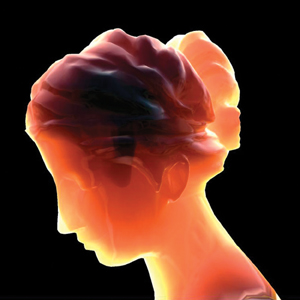
\includegraphics[width=0.3\textwidth]{subsurface-scattering}
  \caption[Subsurface Scattering]{Subsurface Scattering (from \cite{fernando2004gpu})}
  \label{fig:subscat}
\end{figure}

Both of these can be simulated well by Photon Mapping algorithms, although a high amount of caustics will hinder performance considerably.

\end{document}
